\documentclass[a4paper,11pt,dvipsnames,addpoints]{exam}

\usepackage[english]{babel}
% Fonts %
\usepackage{fouriernc}
\usepackage[T1]{fontenc}

% Colors & Graphics %
\usepackage{xcolor}
\usepackage{graphicx}
\graphicspath{ {exam_figs/} }

% Tikz
\usepackage{tikz}
\usetikzlibrary{patterns}
\usepackage{tkz-euclide}

% Figures
\usepackage{float}
\usepackage{caption}
\usepackage{subcaption}

% Page Layout %
\usepackage[margin=1in]{geometry}

\pagestyle{headandfoot}
\firstpageheader{}{}{}
\runningfooter{}{}{}
\runningheader{Exam A}{Page~\thepage~of~\numpages}{\today}
\runningheadrule

% Math stuff %
\usepackage{amsmath}
\usepackage{amssymb}

% Fancy Headers %
\usepackage{enumitem}

% Tables %
\usepackage{booktabs}
\usepackage{tabularx}

\newcommand{\clr}{\textcolor{BrickRed}}
\newcommand{\clb}{\textcolor{RoyalBlue}}
\newcommand{\clg}{\textcolor{ForestGreen}}
\newcommand{\clf}{\textcolor{Fuchsia}}

% Rename solution
\setlength{\fboxsep}{8pt}

% Document %
\begin{document}
\marginpointname{~\%}
\bracketedpoints
\pointsinrightmargin

\begin{center}
 \Huge\sffamily Convex Polygons and Their Symmetries\\[4pt]
 \Large\sffamily 3.AB PreIB Maths -- Exam A
\end{center}

\begin{center}
\framebox{%
 \parbox{.7\textwidth}{%
  \centering
  Unless specified otherwise, you are to \textbf{\clr{always}} (at least
  briefly) explain your reasoning. Even in closed questions.
 }
}
\end{center}
\begin{questions}
 \question Definition of a polygon.
 \begin{parts}
  \part[10] Which of these polygons \emph{\clr{are not}} convex?
  \textbf{Explain}.
  \begin{figure}[H]
   \centering
   \begin{subfigure}[b]{.2\textwidth}
    \centering
    \includegraphics[width=\textwidth]{not_convex_1}
    \caption*{Option A.}
   \end{subfigure}
   \hfill
   \begin{subfigure}[b]{.2\textwidth}
    \centering
    \includegraphics[width=\textwidth]{not_convex_2}
    \caption*{Option B.}
   \end{subfigure}
   \hfill
   \begin{subfigure}[b]{.2\textwidth}
    \centering
    \includegraphics[width=\textwidth]{convex_1}
    \caption*{Option C.}
   \end{subfigure}
   \hfill
   \begin{subfigure}[b]{.2\textwidth}
    \centering
    \includegraphics[width=\textwidth]{convex_2}
    \caption*{Option D.}
   \end{subfigure}
  \end{figure}
  \vspace{2in}
  \part[10] The area of an isosceles (rovnoramenný) triangle with base $\clb{b}$
  and the opposite angle $\clg{\theta}$ (see the picture below) is equal to
  \[
   A = \frac{b^2 \cdot \cos^2 \left( \frac{\theta}{2} \right)}{2 \cdot
   \sin\theta}.
  \]
  Use this fact to calculate the \emph{\clr{area}} of the regular hexagon with
  \emph{\clr{side length $1$}}. \emph{Hint:} $\sin 60^{ \circ } = \cos 30^{
  \circ } = \frac{\sqrt{3}}{2}$.
  \begin{figure}[H]
   \centering
   \begin{subfigure}[b]{.4\textwidth}
    \centering
    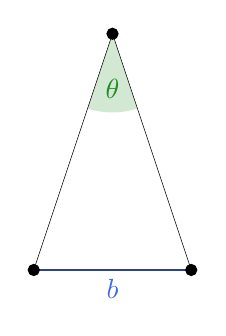
\begin{tikzpicture}
     \tkzInit
     \tkzDefPoints{0/0/a,2/0/b,1/3/c}
     \tkzDrawSegment[thick,RoyalBlue](a,b)
     \tkzLabelSegment[below,RoyalBlue](a,b){$b$}
     \tkzFillAngle[size=1,fill=ForestGreen!20](a,c,b)
     \tkzLabelAngle[ForestGreen,yshift=3mm](a,c,b){$\theta$}

     \tkzDrawPoints[size=4,fill=black](a,b,c)
     \tkzDrawPolygon(a,b,c)
    \end{tikzpicture}
   \end{subfigure}
   \begin{subfigure}[b]{.4\textwidth}
    \centering
    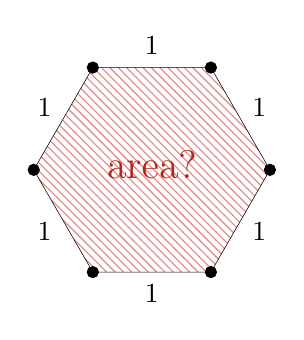
\begin{tikzpicture}[scale=1.5]
     \tkzInit
     \foreach \n/\a in {1/0,2/60,3/120,4/180,5/240,6/300} {
      \tkzDefPoint(\a:1){\n}
     }
     \foreach \a in {30,90,...,330} {
      \node at (\a:1.05) {$1$};
     }
     \tkzDrawPolygon[pattern=north west lines,pattern
     color=BrickRed!40](1,2,3,4,5,6)
     \tkzDrawPoints[size=4,fill=black](1,2,3,4,5,6)
     \node[baseline=.5ex] at (0,0) {\strut\Large\clr{area?}};
    \end{tikzpicture}
   \end{subfigure}
  \end{figure}
  \clearpage
 \end{parts}

 \question Triangulations of convex polygons.
 \begin{parts}
  \part[10] Draw all triangulations of the heptagon \emph{\clr{that can be
  reached in one flip}} from the one shown below. Use the provided shapes (not
  all of them necessarily). \textbf{No explanation required}.
  \begin{figure}[H]
   \centering
   \includegraphics[width=.15\textwidth]{hepta_triangulation}

   \caption*{The initial triangulation.}
  \end{figure}
  \begin{figure}[H]
   \centering
   \begin{subfigure}[b]{.3\textwidth}
    \centering
    \includegraphics[width=.5\textwidth]{hepta_plain}
   \end{subfigure}
   \begin{subfigure}[b]{.3\textwidth}
    \centering
    \includegraphics[width=.5\textwidth]{hepta_plain}
   \end{subfigure}
   \begin{subfigure}[b]{.3\textwidth}
    \centering
    \includegraphics[width=.5\textwidth]{hepta_plain}
   \end{subfigure}
  \end{figure}
  \begin{figure}[H]
   \centering
   \begin{subfigure}[b]{.3\textwidth}
    \centering
    \includegraphics[width=.5\textwidth]{hepta_plain}
   \end{subfigure}
   \begin{subfigure}[b]{.3\textwidth}
    \centering
    \includegraphics[width=.5\textwidth]{hepta_plain}
   \end{subfigure}
   \begin{subfigure}[b]{.3\textwidth}
    \centering
    \includegraphics[width=.5\textwidth]{hepta_plain}
   \end{subfigure}
   \caption*{Shapes to draw diagonals into.}
  \end{figure}
  \part[10] The `formal' definition of a \emph{flip} I gave goes like this:
  \emph{To flip a diagonal, choose a quadrilateral containing this diagonal and
   such that it does not intersect any other diagonals of the triangulation.
   Swap this diagonal for the other one of this quadrilateral}. There is always
   \emph{\clr{exactly one}} correct choice of this quadrilateral. However,
   \emph{\clr{how many}} choices of such a quadrilateral \emph{\clr{are wrong}}
   in a convex polygon on $n$ vertices? Is the number the same for
  \emph{\clr{every}} diagonal?
   \begin{figure}[H]
    \centering
    \begin{subfigure}[b]{.3\textwidth}
     \centering
     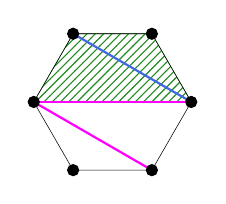
\begin{tikzpicture}
      \tkzInit
      \foreach \n/\a in {1/0,2/60,3/120,4/180,5/240,6/300} {
       \tkzDefPoint(\a:1){\n}
      }
      \tkzDrawPolygon[draw=ForestGreen,pattern=north east lines,pattern
      color=ForestGreen](1,2,3,4)
      \tkzDrawSegments[thick,Fuchsia](1,4 4,6)
      \tkzDrawSegment[thick,RoyalBlue](1,3)

      \tkzDrawPoints[size=4,fill=black](1,2,3,4,5,6)
      \tkzDrawPolygon(1,2,3,4,5,6)
     \end{tikzpicture}
     \caption*{\clg{Correct} quadrilateral.}
    \end{subfigure}
    \begin{subfigure}[b]{.3\textwidth}
     \centering
     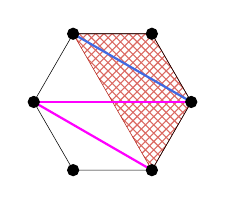
\begin{tikzpicture}
      \tkzInit
      \foreach \n/\a in {1/0,2/60,3/120,4/180,5/240,6/300} {
       \tkzDefPoint(\a:1){\n}
      }
      \tkzDrawPolygon[draw=BrickRed,pattern=crosshatch,pattern
      color=BrickRed!50](1,2,3,6)
      \tkzDrawSegments[thick,Fuchsia](1,4 4,6)
      \tkzDrawSegment[thick,RoyalBlue](1,3)

      \tkzDrawPoints[size=4,fill=black](1,2,3,4,5,6)
      \tkzDrawPolygon(1,2,3,4,5,6)
     \end{tikzpicture}
     \caption*{\clr{Incorrect} quadrilateral.}
    \end{subfigure}
    \begin{subfigure}[b]{.3\textwidth}
     \centering
     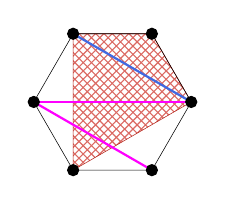
\begin{tikzpicture}
      \tkzInit
      \foreach \n/\a in {1/0,2/60,3/120,4/180,5/240,6/300} {
       \tkzDefPoint(\a:1){\n}
      }
      \tkzDrawPolygon[draw=BrickRed,pattern=crosshatch,pattern
      color=BrickRed!50](1,2,3,5)
      \tkzDrawSegments[thick,Fuchsia](1,4 4,6)
      \tkzDrawSegment[thick,RoyalBlue](1,3)

      \tkzDrawPoints[size=4,fill=black](1,2,3,4,5,6)
      \tkzDrawPolygon(1,2,3,4,5,6)
     \end{tikzpicture}
     \caption*{\clr{Incorrect} quadrilateral.}
    \end{subfigure}
    \caption*{A \clf{triangulation} of the hexagon. The \clb{blue} diagonal
     belongs to three different quadrilaterals. However, only the \clg{green} one
     leads to a correct flip.}
   \end{figure}
  \end{parts}
 \clearpage
 \question Plane transformations.
 \begin{parts}
  \part[10] Find out the \emph{\clg{image}} (the resulting shape when
  transformed) of a square (depicted below) under the plane transformation
  $\clb{f}(x,y) = (2x,y)$. \textbf{Provide a short explanation}.
  \begin{figure}[H]
   \centering
   \begin{subfigure}[c]{.3\textwidth}
    \centering
    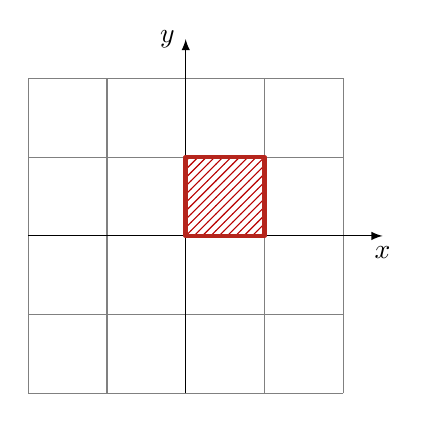
\begin{tikzpicture}
     \tkzInit[xmin=-2,xmax=2,ymin=-2,ymax=2]
     \tkzGrid
     \tkzDrawX
     \tkzDrawY
     \tkzDefPoints{0/0/a,0/1/b,1/1/c,1/0/d}
     \tkzDrawPolygon[ultra thick,BrickRed,pattern={north east lines}, pattern
     color=BrickRed](a,b,c,d)
    \end{tikzpicture}
    \caption*{The initial \clr{square}.}
   \end{subfigure}
   \hspace*{-2em}
   \begin{subfigure}[b]{.3\textwidth}
    \centering
    \begin{tikzpicture}
     \node (origin) at (0,0) {};
     \draw[-latex,thick,bend left=30,RoyalBlue] (0,1) to
      node[midway,yshift=3mm]{$f$} (4,1);
    \end{tikzpicture}
   \end{subfigure}
   \begin{subfigure}[c]{.3\textwidth}
    \centering
    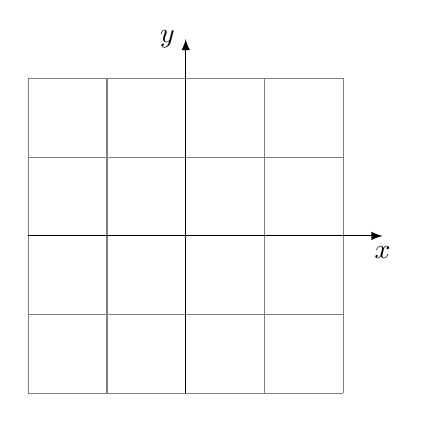
\begin{tikzpicture}
     \tkzInit[xmin=-2,xmax=2,ymin=-2,ymax=2]
     \tkzGrid
     \tkzDrawX
     \tkzDrawY
    \end{tikzpicture}
    \caption*{Draw the resulting shape here.}
   \end{subfigure}
  \end{figure}
  \vspace{2in}
  \part[10] Below, you see a unit \clr{square} transformed by the plane
  transformation $\clg{f}$ defined as $\clg{f}(x,y) = (2 - x - y, 1 - y)$. Write
  this transformation as a composition $\clb{g} \circ s$ (that is, first goes
  $s$, then goes $\clb{g}$) where $s$ is a symmetry of the \clr{square}
  (applying it keeps the square intact). \textbf{Explain}.
  \begin{figure}[H]
   \centering
   \begin{subfigure}[c]{.3\textwidth}
    \centering
    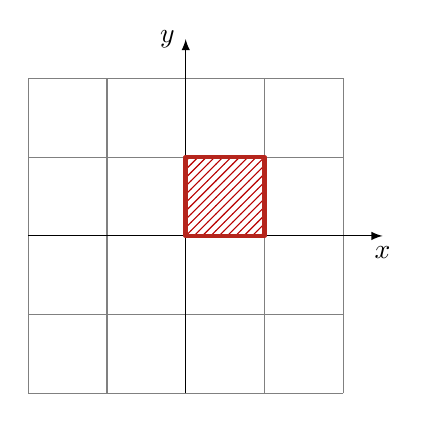
\begin{tikzpicture}
     \tkzInit[xmin=-2,xmax=2,ymin=-2,ymax=2]
     \tkzGrid
     \tkzDrawX
     \tkzDrawY
     \tkzDefPoints{0/0/a,0/1/b,1/1/c,1/0/d}
     \tkzDrawPolygon[ultra thick,BrickRed,pattern={north east lines}, pattern
     color=BrickRed](a,b,c,d)
    \end{tikzpicture}
    \caption*{The \clr{initial} square.}
   \end{subfigure}
   \hspace*{-2em}
   \begin{subfigure}[b]{.3\textwidth}
    \centering
    \begin{tikzpicture}
     \node (origin) at (0,0) {};
     \draw[-latex,thick,bend left=30,ForestGreen] (0,1) to
      node[midway,yshift=3mm]{$g$} (4,1);
    \end{tikzpicture}
   \end{subfigure}
   \begin{subfigure}[c]{.3\textwidth}
    \centering
    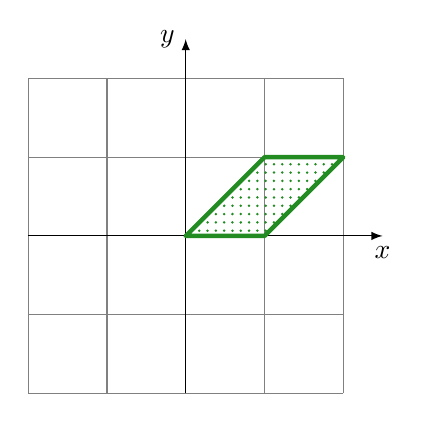
\begin{tikzpicture}
     \tkzInit[xmin=-2,xmax=2,ymin=-2,ymax=2]
     \tkzGrid
     \tkzDrawX
     \tkzDrawY
     \tkzDefPoints{0/0/a,1/0/b,1/1/c,2/1/d}
     \tkzDrawPolygon[ultra thick,ForestGreen,pattern={dots}, pattern
     color=ForestGreen](a,b,d,c)
    \end{tikzpicture}
   \caption*{The square transformed by $\clg{f}$.}
   \end{subfigure}
  \end{figure}
 \end{parts}
 \clearpage
 \question Symmetries of regular polygons.
 \begin{parts}
  \part[10] Given two symmetries of the \emph{square} -- the rotation $\clr{r} =
  ~\circlearrowleft 270^{ \circ }$ by $270^{ \circ }$ counter-clockwise and the
  reflection $\clb{s}$ drawn below -- determine (using any method you wish) the
  composition $\clb{s}\clr{r}$. \textbf{Explain}.
  \begin{center}
   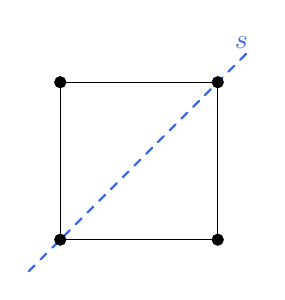
\begin{tikzpicture}[scale=2]
    \tkzInit
    \tkzDefPoints{0/0/a,0/1/b,1/1/c,1/0/d}
    \tkzDrawLine[thick,dashed,RoyalBlue](a,c)
    \tkzLabelLine[pos=1.2,yshift=1mm,xshift=-1mm](a,c){$\clb{s}$}
    \tkzDrawPoints[size=4,fill=black](a,b,c,d)
    \tkzDrawPolygon(a,b,c,d)
   \end{tikzpicture}
  \end{center}
  \vspace{2in}
  \part[10] Given two symmetries of the octakaidecagon (18 vertices) -- the
  reflections $\clr{s_1}$ and $\clb{s_2}$ depicted below -- compute (using any
  method you wish) the composition $\clr{s_1}\clb{s_2}$. \textbf{Explain}.
  \begin{figure}[H]
   \centering
   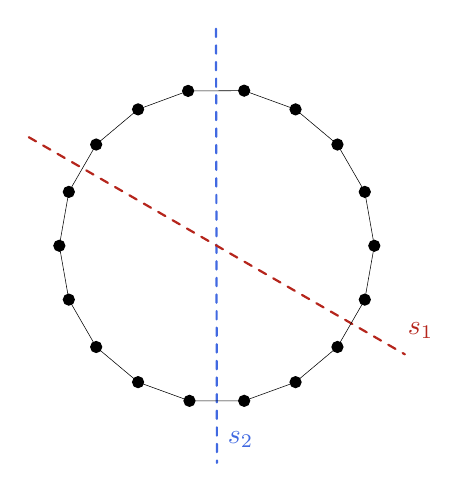
\begin{tikzpicture}[scale=2]
    \tkzInit
    \foreach \n/\a in
    {1/20,2/40,3/60,4/80,5/100.5,6/120,7/140,8/160,9/180,10/200,
    11/220,12/240,13/260,14/280,15/300,16/320,17/340,18/0} {%
     \tkzDefPoint(\a:1){\n}
    }
    \foreach \n in {1,2,...,18}{%
     \tkzDrawPoint[size=4,fill=black](\n)
    }
    \tkzDefMidPoint(4,5)\tkzGetPoint{m1}
    \tkzDefMidPoint(13,14)\tkzGetPoint{m2}
    \tkzDefMidPoint(7,8)\tkzGetPoint{m3}
    \tkzDefMidPoint(16,17)\tkzGetPoint{m4}
    \tkzDrawLine[thick,dashed,RoyalBlue](m1,m2)
    \tkzDrawLine[thick,dashed,BrickRed](m3,m4)
    \tkzLabelLine[pos=1.2,yshift=3mm,xshift=3mm](m1,m2){$\clb{s_2}$}
    \tkzLabelLine[pos=1.2,yshift=3mm,xshift=2mm](m3,m4){$\clr{s_1}$}
    \tkzDrawPolygon(1,2,3,4,5,6,7,8,9,10,11,12,13,14,15,16,17,18)
   \end{tikzpicture}
  \end{figure}
  \clearpage
  \part[10] Select those of the following four pairs of symmetries of the
  regular enneagon (9 vertices) that \emph{\clr{generate all}} of its
  symmetries. \textbf{No explanation necessary}.
  \begin{figure}[H]
   \centering
   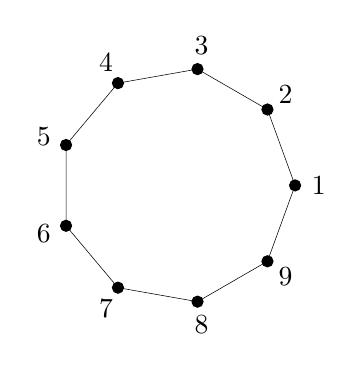
\begin{tikzpicture}[scale=1.5]
    \foreach \n/\a in {
     1/0.00,2/40.00,3/80.00,4/120.00,5/160.00,6/200.00,7/240.00,8/280.00,9/320.00
     } {
      \tkzDefPoint(\a:1){\n}
      \tkzDrawPoint[size=4,fill=black](\n)
      \node at (\a:1.2) {$\n$};
     }
     \tkzDrawPolygon(1,2,3,4,5,6,7,8,9)
   \end{tikzpicture}
   \caption*{Picture of the enneagon for reference.}
  \end{figure}
  \begin{checkboxes}
   \item the rotation $\clr{r_1} =~\circlearrowleft 4 \cdot 360^{ \circ } / 9$ and
    the rotation $\clr{r_2} = ~\circlearrowleft 8 \cdot 360^{ \circ } / 9$,
   \item the reflection $\clb{s_1}$ over the line passing through vertex $6$ and
    the midpoint of $12$ and the reflection $\clb{s_2}$ over the line passing
    through vertex $3$ and the midpoint of $78$.
   \item the reflection $\clb{s}$ over the line passing through vertex $1$ and
    the midpoint of $56$ and the rotation $\clr{r} = ~\circlearrowleft 6 \cdot
    360^{ \circ } / 9$,
   \item the rotation $\clr{r} =~\circlearrowleft 7 \cdot 360^{ \circ } / 9$ and
    the reflection $\clb{s}$ over the line passing through vertex $8$ and the
    midpoint of $34$.
  \end{checkboxes}
  \part[10] Given reflections $\clr{s_1}$ and $\clb{s_2}$ of the heptagon (7
  vertices), compose them (and \emph{\clr{only}} them) to create the reflection
  $\clg{s_3}$ illustrated below. \textbf{Explain}.
  \begin{center}
   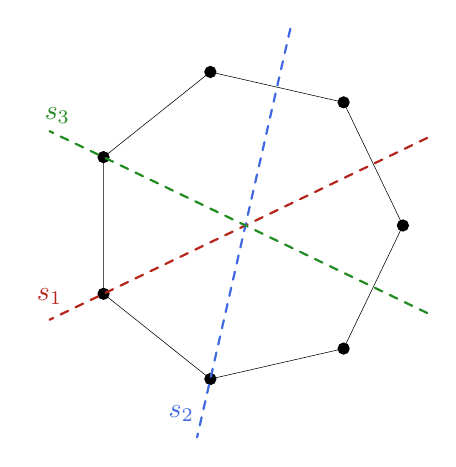
\begin{tikzpicture}[scale=2]
    \foreach \n/\a in {
     1/0.00,2/51.43,3/102.86,4/154.29,5/205.71,6/257.14,7/308.57
     } {
      \tkzDefPoint(\a:1){\n}
      \tkzDrawPoint[size=4,fill=black](\n)
     }
     \tkzDrawPolygon(1,2,3,4,5,6,7)
     \tkzDefMidPoint(1,2)\tkzGetPoint{m1}
     \tkzDefMidPoint(2,3)\tkzGetPoint{m2}
     \tkzDrawLine[thick,dashed,BrickRed](m1,5)
     \tkzDrawLine[thick,dashed,RoyalBlue](m2,6)
     \tkzLabelLine[pos=1.2,yshift=3mm](m1,5){$\clr{s_1}$}
     \tkzLabelLine[pos=1.2,yshift=3mm,xshift=-2mm](m2,6){$\clb{s_2}$}

     \tkzDefMidPoint(1,7)\tkzGetPoint{m3}
     \tkzDrawLine[thick,dashed,ForestGreen](m3,4)
     \tkzLabelLine[pos=1.2,xshift=1mm,yshift=2mm](m3,4){$\clg{s_3}$}
   \end{tikzpicture}
  \end{center}
 \end{parts}
\end{questions}

\end{document}
